%! TEX root = self_chapter-4.tex

\setcounter{chapter}{3}
\chapter{Hasil dan Pembahasan}

\def\True{\mathtt{True}}
\def\False{\mathtt{False}}
\def\min{\mathtt{min}}
\def\Bbb{\mathbb{B}}
\renewcommand{\foreign}[1]{\foreignlanguage{english}{\textit{#1}}}

\section{Landasan Formal}

Untuk mempermudah pembahasan, terlebih dahulu didefinisikan beberapa notasi. Misalkan \(S\) merupakan suatu himpunan sembarang. Sebuah vektor berdimensi \(n\) yang elemennya berasal dari \(S\) ditulis sebagai \(c \in S^n\), dengan \(c_i \in S\) menyatakan elemen ke-\(i\) dari vektor tersebut. Vektor \(c\) dapat dibangun dari elemen-elemennya dengan notasi \(c = (c_1\ \cdots\ c_n)\), atau secara singkat \(c = (c_i\ \cdots)\) ketika domain indeks \(i\) jelas dari konteks.

Selanjutnya, sebuah matriks \(A\) berukuran \(m\) baris dan \(n\) kolom yang elemennya berasal dari \(S\) ditulis sebagai \(A \in S^{m\times n}\), dengan \(A_{ij} \in S\) menyatakan elemen di baris ke-\(i\) dan kolom ke-\(j\) dari matriks tersebut. Digunakan notasi \(A_{*j} \in S^m\) untuk kolom ke-\(j\) dan \(A_{i*} \in S^n\) untuk baris ke-\(i\).

Kemudian, misalnya, diberikan \(a_1,\ \cdots,\ a_m \in S^n\). Sebuah matriks \(A \in S^{n\times m}\) dapat dibangun dengan menyusun vektor-vektor tersebut secara bersampingan, yaitu \(A = [a_1\ \cdots\ a_m]\), atau secara singkat \(A = [a_i\ \cdots]\) ketika domain indeks \(i\) jelas dari konteks. Demikian pula, sebuah matriks \(A \in S^{m\times n}\) dapat dibangun dengan menyusun vektor-vektor tersebut secara bertumpuk, yaitu
	\[ A = \left[ \begin{array}{c} a_1\\ \vdots\\ a_m \end{array} \right], \quad \text{atau secara singkat } A = \left[ \begin{array}{c} a_i\\ \vdots \end{array} \right] \text{.}\]

Dengan demikian, matriks \(A\) dapat dibangun dari elemen-elemen barisnya maupun dari elemen-elemen kolomnya sebagai berikut.
	\[ A = \left[ \begin{array}{c} A_{i*}\\ \vdots \end{array} \right] = [A_{*j}\ \cdots] \]

Selanjutnya, didefinisikan sebuah operator boolean biner sebagai operasi yang memetakan dua unsur ke dalam nilai boolean \(\Bbb = \{\True, \False\}\). Untuk setiap \(s_1, s_2 \in S\), didefinisikan \((s_1 = s_2) \in \Bbb\) sebagai berikut.
	\[ (s_1 = s_2) = \left\{
	\begin{array}{l@{\ }l}
		\True  &\iff s_1 = s_2 \\
		\False &\iff s_1 \neq s_2
	\end{array} \right. \]
Secara natural, operator tersebut dapat diperluas untuk \(a, b \in S^n\), sehingga \((a = b) \in \Bbb^n\) merupakan vektor boolean yang komponennya diberikan oleh \((a = b)_i = (a_i = b_i)\), dan oleh karena itu \((a = b) = ((a_i = b_i)\ \cdots)\).

\cleardoublepage

Didefinisikan sebuah operator boolean biner lain yang berbentuk \((s_1 | s_2) \in \Bbb\) untuk \(s_1, s_2 \in S\) sebagai berikut.
	\[ (s_1 = s_2) = \left\{
	\begin{array}{l@{\ }l@{\ }c}
		\True  &\iff& s_1 \vee s_2 \\
		\False &\iff& \neg s_1 \wedge \neg s_2
	\end{array} \right. \]
Seperti sebelumnya, operator ini diperluas untuk \(a, b \in S^n\) dengan \((a | b) = ((a_i | b_i)\ \cdots) \in \Bbb^n\).

Terakhir, diperkenalkan beberapa notasi yang berhubungan dengan graf. Misalkan \(G\) adalah graf. Representasi graf \(G\) dalam bentuk matriks ketetanggaan ditulis sebagai \(M\). Untuk \(V\), himpunan seluruh simpul di \(G\), matriks jarak simpul ke simpul dari \(G\) ditulis sebagai \(D^{(V)}\), sehingga jarak antar dua simpul \(v_i,v_j \in V\) adalah \(d(v_i,v_j) = D_{i,j}^{(V)}\). Untuk \(E\), himpunan seluruh sisi di \(G\), matriks jarak simpul ke sisi dari \(G\) ditulis sebagai \(D^{(E)}\), sehingga jarak antara simpul \(v_i \in V\) dan sisi \(e_j \in E\) adalah \(d(v_i,e_j) = D_{i,j}^{(E)}\).

Dengan menggunakan notasi yang telah didefinikan, perhatikan bahwa matriks jarak simpul ke simpul dapat dibangun melalui representasi, yaitu \(D = [r(v_i|V)\ \cdots]\), karena \(r(u|V) = (d(u,v_j)\ \cdots), v_j \in V\). Demikian pula, matriks jarak simpul ke sisi dapat dibangun melalui representasi, yaitu \(D = [r(e_i|V)\ \cdots]\), karena \(r(e,v_j) = (d(e,v_j)\ \cdots), v_j \in V\).

\section{Formulasi Algoritma}

Pondasi yang digunakan oleh seluruh formulasi algoritma di sini adalah matriks yang bernama \foreign{distance similarity matrix} untuk penentuan dimensi metrik, atau \foreign{edge distance similarity matrix} untuk penentuan dimensi metrik sisi. Untuk membangun masing-masing matriks tersebut, diperlukan matriks jarak simpul ke simpul dan matriks jarak simpul ke sisi.

Oleh karena itu, \foreign{input} yang digunakan adalah representasi matriks ketetanggaan \(M\) dari graf \(G\). Kemudian, \(D^{(V)}\) dapat dikonstruksi dari \(M\) menggunakan algoritma \foreign{Floyd-Warshall}. Dan \(D^{(E)}\) dapat dikonstruksi langsung dari definisi jarak simpul ke sisi; yaitu jarak dari simpul \(v_i \in V\) ke sisi \(e_j \in E\), di mana \(e_j\) adalah sisi yang menghubungkan dua simpul \(v_k, v_l \in V\), adalah \(d(v_i,e_j) = \min(d(v_i, v_k), d(v_i, v_l))\), sehingga \(D_{ij}^{(E)} = \min(D_{ik}^{(V)}, D_{il}^{(V)})\).

\foreign{Distance similarity matrix} dari \(G\) yang dinotasikan \(B^{(V)} \in \Bbb^{|V|\times \frac{|V|(|V|-1)}{2}}\) dan \foreign{edge distance similarity matrix} dari \(G\) yang dinotasikan \(B^{(E)} \in \Bbb^{|V|\times \frac{|E|(|E|-1)}{2}}\) berturut-turut merupakan hasil dari perbandingan antara setiap kolom berbeda di \(D^{(V)}\) serta \(D^{(E)}\).
	\[ B^{(V)} = [(D_{*j}^{(V)} = D_{*k}^{(V)})\ \cdots], \quad j < k\]
	\[ B^{(E)} = [(D_{*j}^{(E)} = D_{*k}^{(E)})\ \cdots], \quad j < k\]

Kemudian, dari \(B^{(V)}\), dikonstruksi matriks yang bernama \foreign{reduced distance similarity}, dan dinotasikan \(P^{(V)}\), atau dari \(B^{(E)}\), dikonstruksi matriks yang bernama \foreign{reduced edge distance similarity}, dan dinotasikan \(P^{(E)}\), menggunakan algoritma berikut.
\begin{enumerate}
	\item Tetapkan \(P := B\).
	\item Untuk setiap \(P_{*j}\) dan \(P_{*k}\) dan \(j \neq k\), hapus \(P_{*j}\) jika \((P_{*j} | P_{*k}) = P_{*k}\).
\end{enumerate}

\cleardoublepage

Sebagai contoh, perhatikan graf berikut.

\begin{figure}[!htbp]
	\centering
	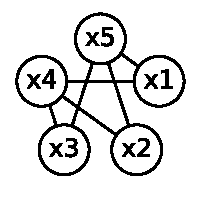
\includegraphics[width=0.25\linewidth]{img/f372738d3845db182fe0b4a3eced9bc2ac778c82a1804f5788cce6bb74ea1beb.pdf}
	\caption{Contoh Graf}
	\label{fig:contoh-graf}
\end{figure}

Graf ini memiliki representasi dalam matriks ketetanggaan sebagai berikut.
\[
	M = \left[ \begin{array}{ccccc}
		0 & 0 & 0 & 1 & 1 \\
		0 & 0 & 0 & 1 & 1 \\
		0 & 0 & 0 & 1 & 1 \\
		1 & 1 & 1 & 0 & 0 \\
		1 & 1 & 1 & 0 & 0
	\end{array} \right]
\]

Menggunakan \foreign{Floyd-Warshall}, didapatkan matriks jarak simpul ke simpul berikut.
\[
	D^{(V)} = \left[ \begin{array}{ccccc}
		0 & 2 & 2 & 1 & 1 \\
		2 & 0 & 2 & 1 & 1 \\
		2 & 2 & 0 & 1 & 1 \\
		1 & 1 & 1 & 0 & 2 \\
		1 & 1 & 1 & 2 & 0
	\end{array} \right]
\]

Selanjutnya, dihasilkan \foreign{distance similarity matrix} berikut.
\[
	B^{(V)} = \left[ \begin{array}{cccccccccc}
		\False & \False & \False & \False &  \True & \False & \False & \False & \False &  \True \\
		\False &  \True & \False & \False & \False & \False & \False & \False & \False &  \True \\
		 \True & \False & \False & \False & \False & \False & \False & \False & \False &  \True \\
		 \True &  \True & \False & \False &  \True & \False & \False & \False & \False & \False \\
		 \True &  \True & \False & \False &  \True & \False & \False & \False & \False & \False
	\end{array} \right]
\]

Kemudian, setelah penghapusan, didapat \foreign{reduced distance similarity} berikut.

\[
	P^{(V)} = \left[ \begin{array}{ccccc}
		\False & \False & \False &  \True &  \True \\
		\False &  \True & \False & \False &  \True \\
		 \True & \False & \False & \False &  \True \\
		 \True &  \True & \False &  \True & \False \\
		 \True &  \True & \False &  \True & \False \\
	\end{array} \right]
\]

\cleardoublepage

\subsection{\foreign{Brute-force}}

...

\subsection{\foreign{Boolean Satisfiability}}

Minimize the number of \(x_i\) that needs to be \(\True\).
\[
	\begin{array}{rl}
		x_3 \vee x_4 \vee x_5 \implies& x_1 \vee x_2 \\
		x_2 \vee x_4 \vee x_5 \implies& x_1 \vee x_3 \\
		& x_1 \vee x_2 \vee x_3 \vee x_4 \vee x_5 \\
		x_1 \vee x_4 \vee x_5 \implies& x_2 \vee x_3 \\
		x_1 \vee x_2 \vee x_3 \implies& x_4 \vee x_5 \\
	\end{array}
\]

\subsection{\foreign{Linear Integer Arithmetic}}

Minimize \(x_1 + x_2 + x_3 + x_4 + x_5 \).
\[
	\begin{array}{r}
		x_1 + x_2 \geq 1 \\
		x_1 + x_3 \geq 1 \\
		x_1 + x_2 + x_3 + x_4 + x_5 \geq 1 \\
		x_2 + x_3 \geq 1 \\
		x_4 + x_5 \geq 1
	\end{array}
\]

\subsection{\foreign{Pseudo Boolean}}

Minimize \(k\).
\[
	\begin{array}{rl}
		x_1 + x_2 + x_3 + x_4 + x_5 &= k\\ [4pt]
		x_3 + x_4 + x_5 &\leq k - 1 \\
		x_2 + x_4 + x_5 &\leq k - 1 \\
		0 &\leq k - 1 \\
		x_1 + x_4 + x_5 &\leq k - 1 \\
		x_1 + x_2 + x_3 &\leq k - 1
	\end{array}
\]

\section{Evaluasi Algoritma}

\section{Pembahasan}
